\documentclass[border=1]{standalone}
\usepackage{tikz}

\begin{document}
    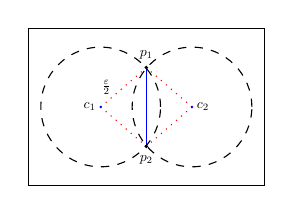
\begin{tikzpicture}
        \draw (0.00, 0.00) rectangle (3.00, 2.00);
        \coordinate (P1) at (1.50, 1.50);
        \coordinate (P2) at (1.50, 0.50);
        \coordinate (C1) at (0.92, 1.00);
        \coordinate (C2) at (2.08, 1.00);
        
        \draw[blue] (P1) -- (P2);
        \draw[dotted, red] (C1) -- node[midway, black, scale=0.5, left=2mm]{$\frac{\varepsilon}{2}$} (P1);
        \draw[dotted, red] (C1) -- (P2);
        \draw[dotted, red] (C2) -- (P1);
        \draw[dotted, red] (C2) -- (P2);
        \node[circle, fill, scale=0.15] at (P1){};
        \node[circle, fill, scale=0.15] at (P2){};
        \node[circle, fill, scale=0.1, color=blue] at (C1){};
        \node[circle, fill, scale=0.1, color=blue] at (C2){};
        \draw[dashed] (C1) circle (0.76);
        \draw[dashed] (C2) circle (0.76);
        
        \node[scale=0.5, above=1mm] at (P1){$p_1$};
        \node[scale=0.5, below=1mm] at (P2){$p_2$};
        \node[scale=0.5, left=0mm] at (C1){$c_1$};
        \node[scale=0.5, right=0mm] at (C2){$c_2$};
    \end{tikzpicture}
\end{document}
